\chapter{Transient heat transfer in solids}
\label{ch:heatcases2}

\subsection{Introduction}
Within the domain of unidirectional heat transfer where the transient evolution
of temperatures is of interest, one can think of two extreme cases. The first
where the heat transfer from the solid is limited by thermal diffusion through
its bulk. This is when the removal of heat from the interface is not
constrained. An example could be a hot ceramic piece kept in front of a fan. 


The second case is when bulk diffusion of heat within the solid is not
constrained at all but the heat transfer at the interface is limited by the
surrounding medium. An example could be a hot copper block kept in still air.


In the second case, one can assume that no thermal gradients would be present
within the solid and use what is known as {\it lumped heat capacitance method}
to obtain the variation of average temperature of the solid with time. This
forms the {\it interface dominated} heat transfer.


In the first case, one needs to solve the equation of thermal diffusion in solid
to determine the thermal gradients that drive the heat flux across the interface
of the solid with the ambient medium. This forms the {\it conduction dominated}
heat transfer.


\subsection{Interface dominated}

The change in the temperature of an object immersed in a fluid at different
temperature can be estimated easily if the thermal conductivity of the object is
high enough that no thermal gradients develop within the object. 

If the characteristic length scale of the object is $L$, we require that the
inner temperature of the object $T_i$ is as close to the surface temperature
$T_s$ as possible. A balance of flux at the surface gives:

$$ k \frac{T_i - T_s}{L} = h \left(T_s - T_\infty\right) $$
or
$$ \frac{T_i - T_s}{T_s - T_\infty} = \frac{hL}{k}$$

We define Biot Number as
$$Bi = \frac{hL}{k}$$

If $Bi \le 0.1$, $T_i$ is close enough to $T_s$ that thermal gradients within
the object can be neglected so that Newtonian cooling is applicable. In such as
case, we can write,

$$ h A \left(T - T_\infty \right) = -\rho C_p V \frac{dT}{dt} $$

$$ \int_{T_0}^{T}{\frac{dT}{T-T_\infty}} = \frac{-hA}{\rho C_p V}
\int_{0}^{t}{dt}$$
or
$$ \ln{\frac{T-T_\infty}{T_0-T_\infty}} = \frac{-hAt}{\rho C_p V}$$
or
$$ \frac{T-T_\infty}{T_0-T_\infty} = \exp{\left(-\frac{hAt}{\rho C_p
V}\right)}$$

Defining $V/A$ as $L$, the characteristic length scale,

$$ \frac{ht}{\rho C_p L} = \frac{hL}{k} \frac{\alpha t}{L^2} = Bi.Fo$$

where, we define Fourier number as:

$$Fo = \frac{\alpha t}{L^2} = \frac{kt}{\rho C_p L^2}$$

Thus, when $Bi \le 0.1$,

$$ \frac{T - T_\infty}{T_0 - T_\infty} = \exp{\left(-Bi.Fo\right)}$$

\begin{figure}[h]
	\begin{center}
		%\framebox{\resizebox{4in}{!}{\includegraphics[bb=0 0 329 425, clip]{images/Bejan_BiFoMap.eps}}}
		\framebox{\resizebox{4in}{!}{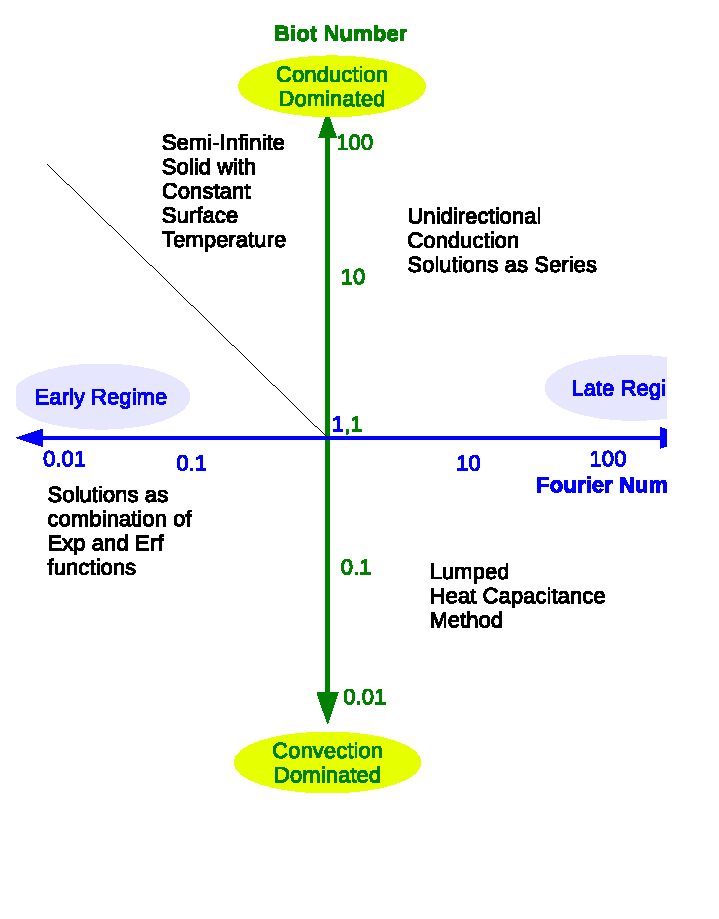
\includegraphics{images/c17-Bejan_BiFoMap.eps}}}
	\end{center}
	\caption{Regimes of domination of convective and conduction heat transfer}
	\label{bejanmap}
\end{figure}


\subsection{Conduction dominated}

In problems where heat transfer is dominated by conduction, temperature as a
function of time and spatial coordinates can be obtained by solving the Fourier
heat conduction equation. 


For the problem of semi-infinite domain where temperature at one end is fixed
and we are interested in its evolution as a function of distance and time, the
governing equation can be written for a one dimensional case as follows.

$$
\label{f2xt}
\frac{\partial T}{\partial t} = \alpha \frac{\partial^2 T}{\partial x^2}
$$

While variable separation is one way of solving this equation, it leads to
summation of a series. We use a co-ordinate transformation to make the equation
simpler.

Put $$\eta = \frac{x}{2\sqrt{\alpha t}}$$ leading to
$$\frac{\partial \eta}{\partial x} = \frac{1}{2\sqrt{\alpha t}}$$
$$\frac{\partial \eta}{\partial t} = \frac{-\eta}{2t}$$
$$\frac{\partial T}{\partial \eta} = \frac{\partial T}{\partial x}
\frac{1}{2\sqrt{\alpha t}}$$
$$\frac{\partial^2 T}{\partial \eta^2} = \frac{\partial^2 T}{\partial x^2}
\frac{1}{4\alpha t}$$


Equation \ref{f2xt} becomes 
$$
\frac{\partial^2 T}{\partial \eta^2} = -2\eta \frac{\partial T}{\partial \eta}
$$
or
$$
\frac{\ddot{T}}{\dot{T}} = -2\eta
$$

Integrating once,
\\
$$
\log\dot{T} = -\eta^2 + \text{constant}
$$
or
$$
\dot{T} = C_1 e^{-\eta^2}
$$
Integrating once more,
$$
T = \int_{\eta=0}^{\eta=\eta}{C_1 e^{-\eta^2} d\eta} + C_2
$$

The integral cannot be simplified and is often given as a tabulated function
with the following definition and properties

$$
\text{erf}(\eta) = \frac{2}{\sqrt{\pi}} \int_{0}^{\eta}{e^{-\eta^2} d\eta}
$$


$$
\frac{\partial}{\partial \eta} \text{erf}(\eta) = \frac{2}{\sqrt{\pi}}
e^{-\eta^2}
$$

$$
\text{erf}(0) = 0
$$

$$
\text{erf}(\infty) = 1
$$

$$
\text{erf}(-\eta) = -\text{erf}(\eta)
$$

Thus, the solution of \ref{f2xt} in a semi-infinite domain can be written as :

$$
\label{erfsol}
\boxed{
T = A \text{erf}(\frac{x}{2\sqrt{\alpha t}}) + B
}
$$

The constants $A$ and $B$ can be determined using the boundary conditions.


\pagebreak

\section{Exercises}

\begin{enumerate}
 \item A long copper wire of 2 mm diameter is exposed to air stream at a
temperature of 400 K. After a minute, the average temperature of the wire
increased from 280 K to 350 K. (a) Estimate the average heat transfer
coefficient on the surface (b) Using the Biot number, comment on the validity of
your solution.

\item Small droplets of a molten glass maintain their amorphicity if they cool
at a rate of atleast \SI{10}{\kelvin\per\second} measured at \SI{1070}{\kelvin}.
For a spherical droplet with \SI{0.1}{\mm} diameter, what is the required heat
transfer coefficient to achieve the minimum cooling rate? The quench environment
is maintained at \SI{293}{\kelvin}. Properties of glass are $\rho$ =
\SI{3000}{\kgpmc}, $C_p$ = \SI{840}{\joule\per\kilo\gram\per\kelvin}, $k$=
\SI{17}{\wpmk}. Verify if your answer is valid for lumped capacitance method to
work.

 \item A typical human body generates about \SI{100}{\watt} due to metabolism.
In order to keep the body temperature at \SI{37}{\celsius}, the heat must be
dissipated through various mechanisms such as convective heat transfer,
radiation, evaporation and conduction that are dynamically balanced depending on
the outside temperature. If the heat loss is significant and the core
temperature drops below \SI{21}{\celsius}, death occurs. Assuming the surface
area of a human body to be about \SI{2}{\meter\squared}, estimate how long a
human can stay alive in (a) quiescent water at \SI{10}{\celsius} where $h$ =
\SI{230}{\wpmsk} and (b) in flowing water at \SI{10}{\celsius} moving at
\SI{0.25}{\mps} where $h$ = \SI{580}{\wpmsk}. Assume $C_p$ of human body to be
about \SI{3470}{\joule\per\kilo\gram\per\kelvin}.

\end{enumerate}


\section{Moving boundary condition}

Problem: Liquid is poured at $T_M$ in a {\em thick} mould kept at $T_0$.
Assuming that all the latent heat is extracted through mould, arrive at the rate
of solidification.

\begin{figure}[h]
\begin{center}
\framebox{
 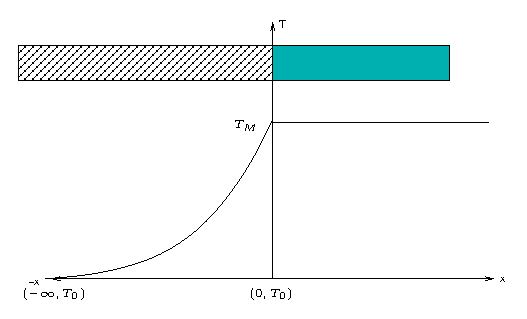
\includegraphics[scale=0.7]{images/c17-ratesolfig.ps}
}
\end{center}
\caption{Temperature profile during solidification}
\label{ratesol1}
\end{figure}

Solution:


\framebox{Solidification is usually antiparallel to the direction of heat
flux}\footnote{Solidification in undercooled melts is an exception}


Heat flux at $x=0$ is 
$$ \vec{J} = -k_m \left. \frac{\partial T}{\partial x} \right|_{x=0} \hat{x}$$

Latent heat release per unit volume of solid formed is $ \rho_s \Delta H_f$

Let the heat transfer be across a constant mould-solid surface area of $A$

Balancing the two,

$$ A J = -\rho_s \Delta H_f \frac{\partial V}{\partial t} $$

since a positive $J$ implies heat flux in $+\hat{x}$ direction leading to a
negative rate of solidification. 

$$
A k_m \left. \frac{\partial T}{\partial x} \right|_{x=0} = \rho_s \Delta H_f
\frac{\partial V}{\partial t}
$$

Writing the error function solution to the temperature in the mould (properties
of mould indicated by subscript $_m$),

$$
\frac{T_M - T}{T_M - T_0} = \text{erf} (\frac{-x}{2\sqrt{\alpha_m t}})
$$

Substituting,

$$
A k_m (T_M - T_0) \frac{2}{\sqrt{\pi}} \frac{1}{2 \sqrt{\alpha_m t}} = \rho_s
\Delta H_f \frac{\partial V}{\partial t} 
$$

or

$$
\frac{1}{A} \frac{\partial V}{\partial t} =  \frac{(T_M - T_0)}{\rho_s \Delta
H_f \sqrt{\pi}} \sqrt{k_m \rho_m C_{pm}} \frac{1}{\sqrt{t}} 
$$

Define {\em heat diffusivity} $H_D$ as 
$$
\boxed{
H_D = \sqrt{k_m \rho_m C_{pm}}
}
$$

Integrating from $V=0$ at $t=0$ to $V=V$ at $t=t$,

$$
\boxed{
\frac{V}{A} =  \frac{2}{\sqrt{\pi}} \frac{(T_M - T_0) {H_D}_m}{\rho_s \Delta
H_f}  \sqrt{t} 
}
$$

{\em Chvorinov's Rule}:
$$
\frac{V}{A} \propto \sqrt{t}
$$

\subsection{Solidification: mould and solid conductivity controlled}

Problem: Liquid at $T_M$ is poured in to a mould at $T_0$. Heat transfer is
controlled by conduction through solid as well as mould. If the mould-solid
interface temperature is $T_S$ after a thickness of $M$ of solid has formed,
derive expressions to estimate the two quantities.

\begin{figure}[h]
\begin{center}
\framebox{
 \includegraphics[scale=0.7]{images/c17-ratesol2fig.ps}
}
\end{center}
\caption{Temperature profile during solidification}
\label{ratesol2}
\end{figure}

Boundary conditions:

BC1: $T=T_0$ at $x=-\infty$ 

BC2: $T=T_S$ at $x=0$ and $t=\tau$

BC3: Flux balance  
$$
-k_m \left. \frac{\partial T}{\partial x} \right|_{x \rightarrow -0} = -k_s
\left. \frac{\partial T}{\partial x} \right|_{x \rightarrow +0}
$$

BC4: $T=T_M$ at $x=M$ and $t=\tau$

BC5: Flux balance
$$
A k_s \left. \frac{\partial T}{\partial x} \right|_{x=M} = \rho_s \Delta H_f
\frac{\partial V}{\partial t}
$$

Solution:

Using BC1 and BC2, write the error function solution for heat conduction in the
mould as:

$$
\frac{T_S - T}{T_S - T_0} = \text{erf} (\frac{-x}{2\sqrt{\alpha_m t}})
$$

Similarly the error function solution for heat conduction in the solid is:

$$
T = A \text{erf}\left(\frac{x}{2\sqrt{\alpha_s t}} \right) + B
$$

Using BC2 and BC4 and naming $\frac{M}{2\sqrt{\alpha_s \tau}}$ as $\phi$, write
the solution for temperature in the solid as

$$
T = T_S + \frac{T_M - T_S}{\text{erf}(\phi)}
\text{erf}\left(\frac{x}{2\sqrt{\alpha_s t}} \right)
$$

BC3 provides an estimate of $T_S$ for a given $\phi$:
$$
k_m \frac{T_S - T_0}{\sqrt{\pi \alpha_m \tau}} = k_s \frac{T_M - T_S}{\sqrt{\pi
\alpha_s \tau}} \frac{1}{\text{erf}(\phi)}
$$

Using the definition of heat diffusivity,

$$
{H_D}_m (T_S - T_0) = \frac{{H_D}_s}{\text{erf}(\phi)} (T_M - T_S) 
$$

Call 

$$
p = \frac{{H_D}_s}{{H_D}_m \text{erf}(\phi)}
$$

$$
\boxed{
T_S = \frac{pT_M + T_0}{p+1}
}
$$

BC5 provides an estimate for $\phi$ as a function of physical parameters.

$$
A k_s \frac{2}{\sqrt{\pi}} e^{-\phi^2} \frac {T_M-T_S}{ \text{erf}(\phi) 2
\sqrt{\alpha_s t} } = \rho_s \Delta H_f \frac{\partial V}{\partial t}
$$

Recognising that $\frac{V}{A} = M$,

$$
k_s \frac{2}{\sqrt{\pi}} e^{-\phi^2} \frac {(T_M-T_S)}{2 \sqrt{\alpha_s t}
\text{erf}(\phi) } = \rho_s \Delta H_f \frac{\partial M}{\partial t}
$$

Integrating the equation from $M=0$ at $t=0$ to $M=M$ at $t=\tau$,

$$
 k_s \frac{2}{\sqrt{\pi}} e^{-\phi^2} \frac {(T_M-T_S)
\sqrt{\tau}}{\sqrt{\alpha_s} \text{erf}(\phi) } = \rho_s \Delta H_f M
$$

Simplifying,

$$
\boxed{
\phi \text{erf}(\phi) e^{\phi^2}  = \frac{C_{ps}(T_M-T_S)}{\Delta H_f
\sqrt{\pi}} 
}
$$

Using a table / plot of $\phi \text{erf}(\phi) e^{\phi^2}$ as a function of
$\phi$, one can look up for the RHS of above equation for the corresponding
$\phi$ which gives the relation $M = 2 \phi \sqrt{\alpha_s \tau}$.

\pagebreak
\section{Exercises}
 
\begin{enumerate}
 \item A two inch slab of aluminium is cast in a mold made of silica sand on one
side and an unknown material on the other side. The cast slab is sectioned to
look at the plane of last solidification that can be identified by porosity. If
it is known that the plane is located \SI{30}{\milli\metre} away from the silica side of
the mould, (a) estimate the heat diffusivity of the unknown mould material. From
the properties of mould materials given below, (b) guess which one comes
closest. Neglect superheat.


Typical values of physical properties:\\
\begin{tabular}{|l|l|l|l|}
\hline
Material & $k$ in\si{\watt\per\metre\per\kelvin} & $\rho$
in\si{\kilo\gram\per\metre\cubed} & $C_p$ in
\si{\joule\per\kilo\gram\per\kelvin} \\
\hline
Silica & 0.6 & 1500 & 1160  \\
Mullite & 0.37 & 1600 & 770  \\
Zircon & 1.0 & 2720 & 840  \\
\hline
\end{tabular}



\item A liquid metal ($L$) at temperatute $T_p$ is poured into a mould ($m$)
kept at temperature $T_0$. (a) If the mould-metal surface reaches thermal
equilibrium instantly, find its temperature $T_s$ when the freezing is yet to
start. (b) A component is formed from an alpha brass alloy poured into a mould
kept at \SI{25}{\celsius}. If the freezing takes place over a temperature range
from \SI{1055}{\celsius} to \SI{1045}{\celsius}, find the minimum pouring
temperature to prevent instantaneous freezing. Properties are as follows. $k_m$
= \SI{1.6}{\wpmk}, $k_L$ = \SI{109}{\wpmk}, $\rho_m$ = \SI{3.2e3}{\kgpmc},
$\rho_L$ = \SI{8.52e3}{\kgpmc}, $C_{p,m}$ =
\SI{1e3}{\joule\per\kilo\gram\per\kelvin}, $C_{p,L}$ =
\SI{385}{\joule\per\kilo\gram\per\kelvin}.

\end{enumerate}
% ----------------------- end of heatcases2.tex --------------------
